\documentclass[a4paper,fleqn]{tufte-handout} 
\usepackage{graphicx}

\title{Computational experiments in Science: Horse wrangling in the digital age}

\author{Mathieu Lagrange and Mathias Rossignol}

%\renewcommand{\baselinestretch}{.88}

\begin{document}

\maketitle

\section{Introduction}

The ready availability of massive amounts of data in numerous scientific fields, while an obvious boon for research, may also occasionally have a pernicious effect, as it lulls scientists into a false sense of confidence in their experimental results. Indeed, while all medical double-blind studies come with the caveat of limited sample size, and no result is considered acquired until it has been consistently duplicated by several teams, computer data analysis studies routinely boast decimal-point precision percentages as proof of the validity of their approach, considering that the size of their experimental dataset guarantees its representativity. Cue subsequent announcements of superior decimal-point precision percentages, in a process we call Progress.

This performance-driven approach to research is probably unavoidable, and it gives evaluation data a crucial importance. A high level of scrutiny is therefore necessary, both of the data themselves and of the way they are used.


\section{Horses spotting}

\begin{marginfigure}
\begin{center}
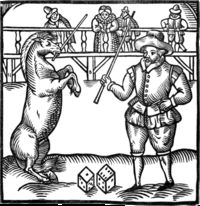
\includegraphics[width=\textwidth]{figures/hans} 
\end{center}
\caption{\label{fig:hans} Hans is clever, but not quite: \url{https://en.wikipedia.org/wiki/Clever_Hans}}
\end{marginfigure}

The data under evaluation in today's challenges are highly multidimensional in many ways: number of dimensions, number of items, number of classes ... Fully understanding the complexity underlying them is more an utopia rather than an achievable goal and as such every drawn conclusion is to be considered with care.

Among many, an issue that arises is the fact that, even if the underlying assumption that helped build a processing chain is correct, the implemented machine may be in fact using other means to achieve the good results we are striving for --~for which the term ``\,horse\,'' has been coined, as a reference to the circus horses that appear to know how to count, but in fact rely on subtle cues (deliberate or subconscious) from their trainer. More precisely, a horse is a system appearing capable of a remarkable human feat but actually working by using irrelevant characteristics (confounds) \cite{6847693}.

Less extreme, more common, and no less concerning, is the phenomenon of ``\,Potemkin villages\,'', or systems that perform extremely well on a given dataset but fail to generalize. Leaving aside the ``\,cherry picking\,'' approach of specifically selecting data to show the system at its best, this can often happen due to a lack of care in ensuring the representativity of the evaluation dataset. This is for example the case in the field of environmental scenes modeling, where the Bag-Of-Frames (BOF) approach\cite{aucouturier2007bag} was long considered as the standard. However, the very good performance of that system is in fact due to a fortunate organization of the dataset\cite{lagrange:hal-01082501}, exhibiting very low intra-class diversity. Evaluated on datasets with realistic intra-class diversity, it completely fails.

Not only do these phenomena lead us to rely on less than satisfactory solutions to open problems, they may also severely stunt progress in the field: the first few publications tackling a given issue establish their dataset and results as \emph{de facto} standards, and promising alternative proposals may be discarded due to their disappointing performance on those same datasets --~but what if the original system was a horse, or the dataset biased?

Thus, our increased reliance on data and evaluation makes it more than ever necessary to exercise care, rigor, doubt and freedom of investigation, which are the cornerstones of the scientific method; and we believe it is crucial to develop tools and processes to that end.

\section{Horse wrangling}

Acknowledging the fact that most of the algorithms we build are probably horses (or Potemkin villages) to a certain degree, we designed some open-source tools that help us better control numerical experiments we have to carry.

\subsection{Data}

\begin{marginfigure}
\begin{center}

\includegraphics[width=\textwidth]{figures/simscene} 
\end{center}
\caption{\label{fig:simScene} SimScene is an open source tool: \url{https://bitbucket.org/mlagrange/simscene}}
\end{marginfigure}

In the field of Acoustic Scene Analysis, evaluation requires large amounts of recorded audio data. Building such datasets is a costly and time-consuming task, and since a large number of factors may vary (nature, density, time positioning and intensity of numerous sound events, background noise\ldots{})
it is practically impossible to record truly representative collections. We have therefore developed \emph{SimScene}, an open-source tool that greatly eases this process by simulating acoustic scenes with a large level of control over their morphology, while making minimal assumptions concerning their structure.

Thanks to it, we can
\begin{enumerate}
\itemsep-.2em 
\item carefully craft evaluation datasets (big is not enough),
\item progressively increase data complexity,
\item isolate factors of complexity,
\item easily share very large amounts of data, by transmitting synthesis parameters instead of actual audio data.
\end{enumerate}

While synthesized audio is still inferior to natural recordings, we believe that the virtually unlimited variations made possible by simScene make it an invaluable research tool to better comprehend the performance of the algorithms under evaluation\cite{lagrange:hal-01111381}.

\subsection{Experimentation}

\begin{marginfigure}
\begin{center}
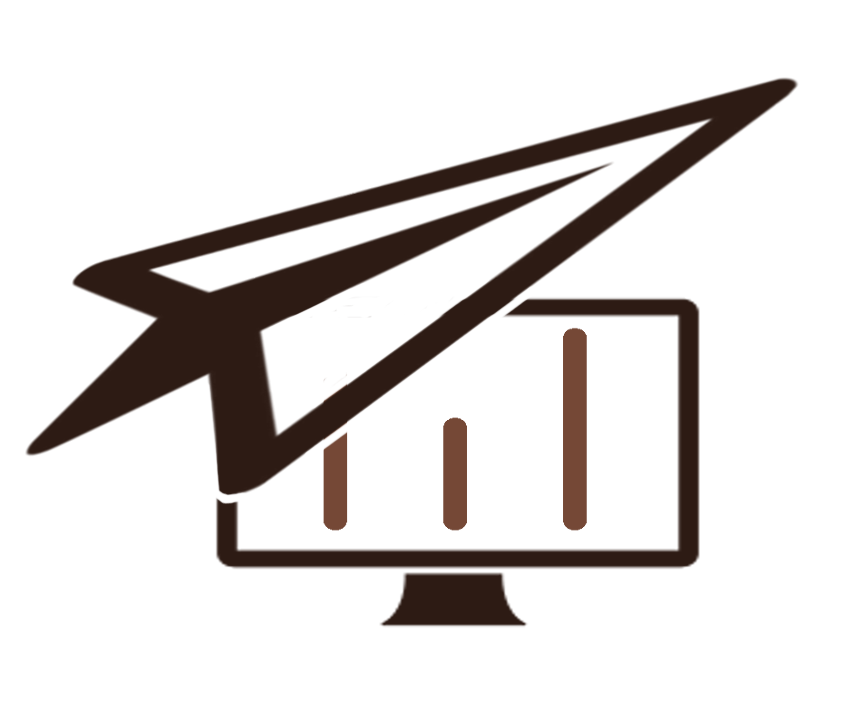
\includegraphics[width=\textwidth]{figures/logo} 
\end{center}
\caption{\label{fig:explanes} ExpLanes is an open source tool: \url{http://mathieulagrange.github.io/expLanes}}
\end{marginfigure}

Algorithms are as complex as the data they process, and measuring their performance is not trivial. Therefore, in our opinion, we shall:
\begin{enumerate}
\itemsep-.2em 
\item thoroughly evaluate the effect of operational parameters,
\item implement lower bound and upper bound baselines,
\item enforce reproducibility, particularly by sharing code.
\end{enumerate}

Moreover, evaluation can be a tedious, time-consuming (``\,do we have time to run another series of tests on this?\,'') and error-prone (``\,were these the exact parameter values I used during the last run?\,'') task. It should therefore be as automated as possible. With those aims in mind, we built an open-source tool called \textsf{expLanes} that greatly eases this process, by proposing a complete evaluation framework that strictly follows the scientific method, and automatically produces synthetic experiment reports.%, see Figure \ref{fig:explanes}.
  
\bibliographystyle{abbrvnat} 
\nobibliography{bib} 
  
\end{document}
